\documentclass[11pt,a4paper]{article}
\usepackage{amsmath,amssymb,amsthm}
\usepackage{graphicx}
\usepackage[margin=2.2cm]{geometry}
\usepackage{xcolor}
\usepackage{titlesec}
\usepackage{fancyhdr}
\usepackage{booktabs}
\usepackage{enumitem}
\usepackage{float}
\usepackage{hyperref}
\hypersetup{colorlinks=true,linkcolor=blue!70!black,urlcolor=blue!70!black}

\renewcommand{\topfraction}{0.9}
\renewcommand{\bottomfraction}{0.9}
\renewcommand{\textfraction}{0.07}
\renewcommand{\floatpagefraction}{0.7}
\setcounter{topnumber}{3}
\setcounter{bottomnumber}{3}
\setcounter{totalnumber}{5}

\definecolor{primary}{RGB}{0,70,140}
\definecolor{accent}{RGB}{204,102,0}

\titleformat{\section}{\Large\bfseries\color{primary}}{\thesection}{1em}{}
\titleformat{\subsection}{\large\bfseries\color{primary!80!black}}{\thesubsection}{1em}{}

\pagestyle{fancy}
\fancyhf{}
\fancyhead[L]{\small\color{primary}Essential Summary}
\fancyhead[R]{\small\color{primary}Li \& Tang (2016)}
\fancyfoot[C]{\thepage}
\renewcommand{\headrulewidth}{0.5pt}

\begin{document}

\begin{center}
{\LARGE\bfseries\color{primary}Essential Summary}\\[12pt]
{\large\bfseries A Generalized Pad\'e--Lindstedt--Poincar\'e Method\\for Predicting Homoclinic and Heteroclinic Bifurcations\\of Strongly Nonlinear Autonomous Oscillators}\\[8pt]
{\normalsize Zhenbo Li, Jiashi Tang}\\[4pt]
{\small\itshape Nonlinear Dynamics, Vol.\ 84, No.\ 3, 1201--1223 (2016)\quad DOI: 10.1007/s11071-015-2563-6}\\[6pt]
{\small\rule{0.7\textwidth}{0.5pt}}\\[4pt]
{\small\color{accent}This is an author-prepared essential summary, not the original paper.\\Please cite the published version.}
\end{center}

\vspace{0.5em}

\section{Background and Motivation}

The Lindstedt--Poincar\'e (L--P) method is a classical perturbation technique for weakly nonlinear oscillators. However, for strongly nonlinear systems---and especially for predicting \textbf{global bifurcations} (homoclinic/heteroclinic)---the traditional L--P method faces two fundamental obstacles: (1) the perturbation procedure requires repeated derivation and integration, which becomes prohibitively cumbersome at high orders for complicated oscillators; and (2) the method was originally designed for periodic solutions, not for the limit-cycle-to-homoclinic transition regime.

This work introduces the \textbf{generalized Pad\'e--Lindstedt--Poincar\'e (GPLP) method}---a synthesis that replaces the integration steps in the L--P procedure with generalized Pad\'e approximation, thereby eliminating the derivation/integration bottleneck while retaining the systematic perturbation framework. This is the foundational paper of the GPLP method, later extended by the authors to more complex oscillators (J.\ Vib.\ Eng.\ Technol., 2022).

\section{Method: GPLP Framework}

\subsection{The Core Idea}

Traditional L--P method steps: (1) introduce nonlinear time transformation $\varphi = \omega t$, (2) expand solution and frequency in powers of $\varepsilon$, (3) solve each-order perturbation equation by \textbf{integration} to eliminate secular terms. Step (3) is the bottleneck---for oscillators with complicated restoring forces, the integrals become intractable.

GPLP replaces step (3) with a \textbf{generalized Pad\'e approximation} procedure:
\begin{enumerate}[leftmargin=2em]
\item Assume the solution to each perturbation order as a generalized Pad\'e approximant (rational function of harmonic functions)
\item Determine its coefficients by matching with the perturbation equation---\textbf{no integration required}
\item The frequency $\omega$ is obtained simultaneously from the matching conditions
\end{enumerate}

\subsection{Generalized Pad\'e Approximants Employed}

Several types of approximants are constructed and tested:
\begin{itemize}[leftmargin=2em]
\item \textbf{Symmetric homoclinic:} $x(\varphi) = \frac{\sum_{i=0}^{m} \alpha_i \cos^{2i}\varphi}{\sum_{j=0}^{n} \beta_j \cos^{2j}\varphi}$ --- exploits symmetry of homoclinic orbits
\item \textbf{Asymmetric heteroclinic:} $x(\varphi) = \frac{\sum_{i=0}^{m} \alpha_i \sin^{2i}\varphi}{\sum_{j=0}^{n} \beta_j \sin^{2j}\varphi}$ --- accommodates asymmetric saddle connections
\item \textbf{Mixed type:} Combinations for oscillators where homoclinic and heteroclinic orbits coexist
\end{itemize}

\subsection{Advantages Over Traditional L--P}

\begin{enumerate}[leftmargin=2em]
\item \textbf{No derivation/integration:} The most time-consuming steps are eliminated. High-order solutions become accessible.
\item \textbf{Handles strong nonlinearity:} Since Pad\'e approximants are global rational functions (not local Taylor expansions), they capture strongly nonlinear behavior well.
\item \textbf{Direct bifurcation prediction:} By treating the bifurcation parameter analytically, the critical homoclinic/heteroclinic values are obtained directly from the amplitude--parameter relation.
\end{enumerate}

\section{Applications}

\subsection{Helmholtz--Duffing Oscillator}

The asymmetric Helmholtz--Duffing oscillator serves as a benchmark for heteroclinic bifurcation prediction. GPLP provides analytical homoclinic/heteroclinic solutions and predicts critical bifurcation parameters (Fig.\ 1).

\begin{figure}[htbp]
\centering
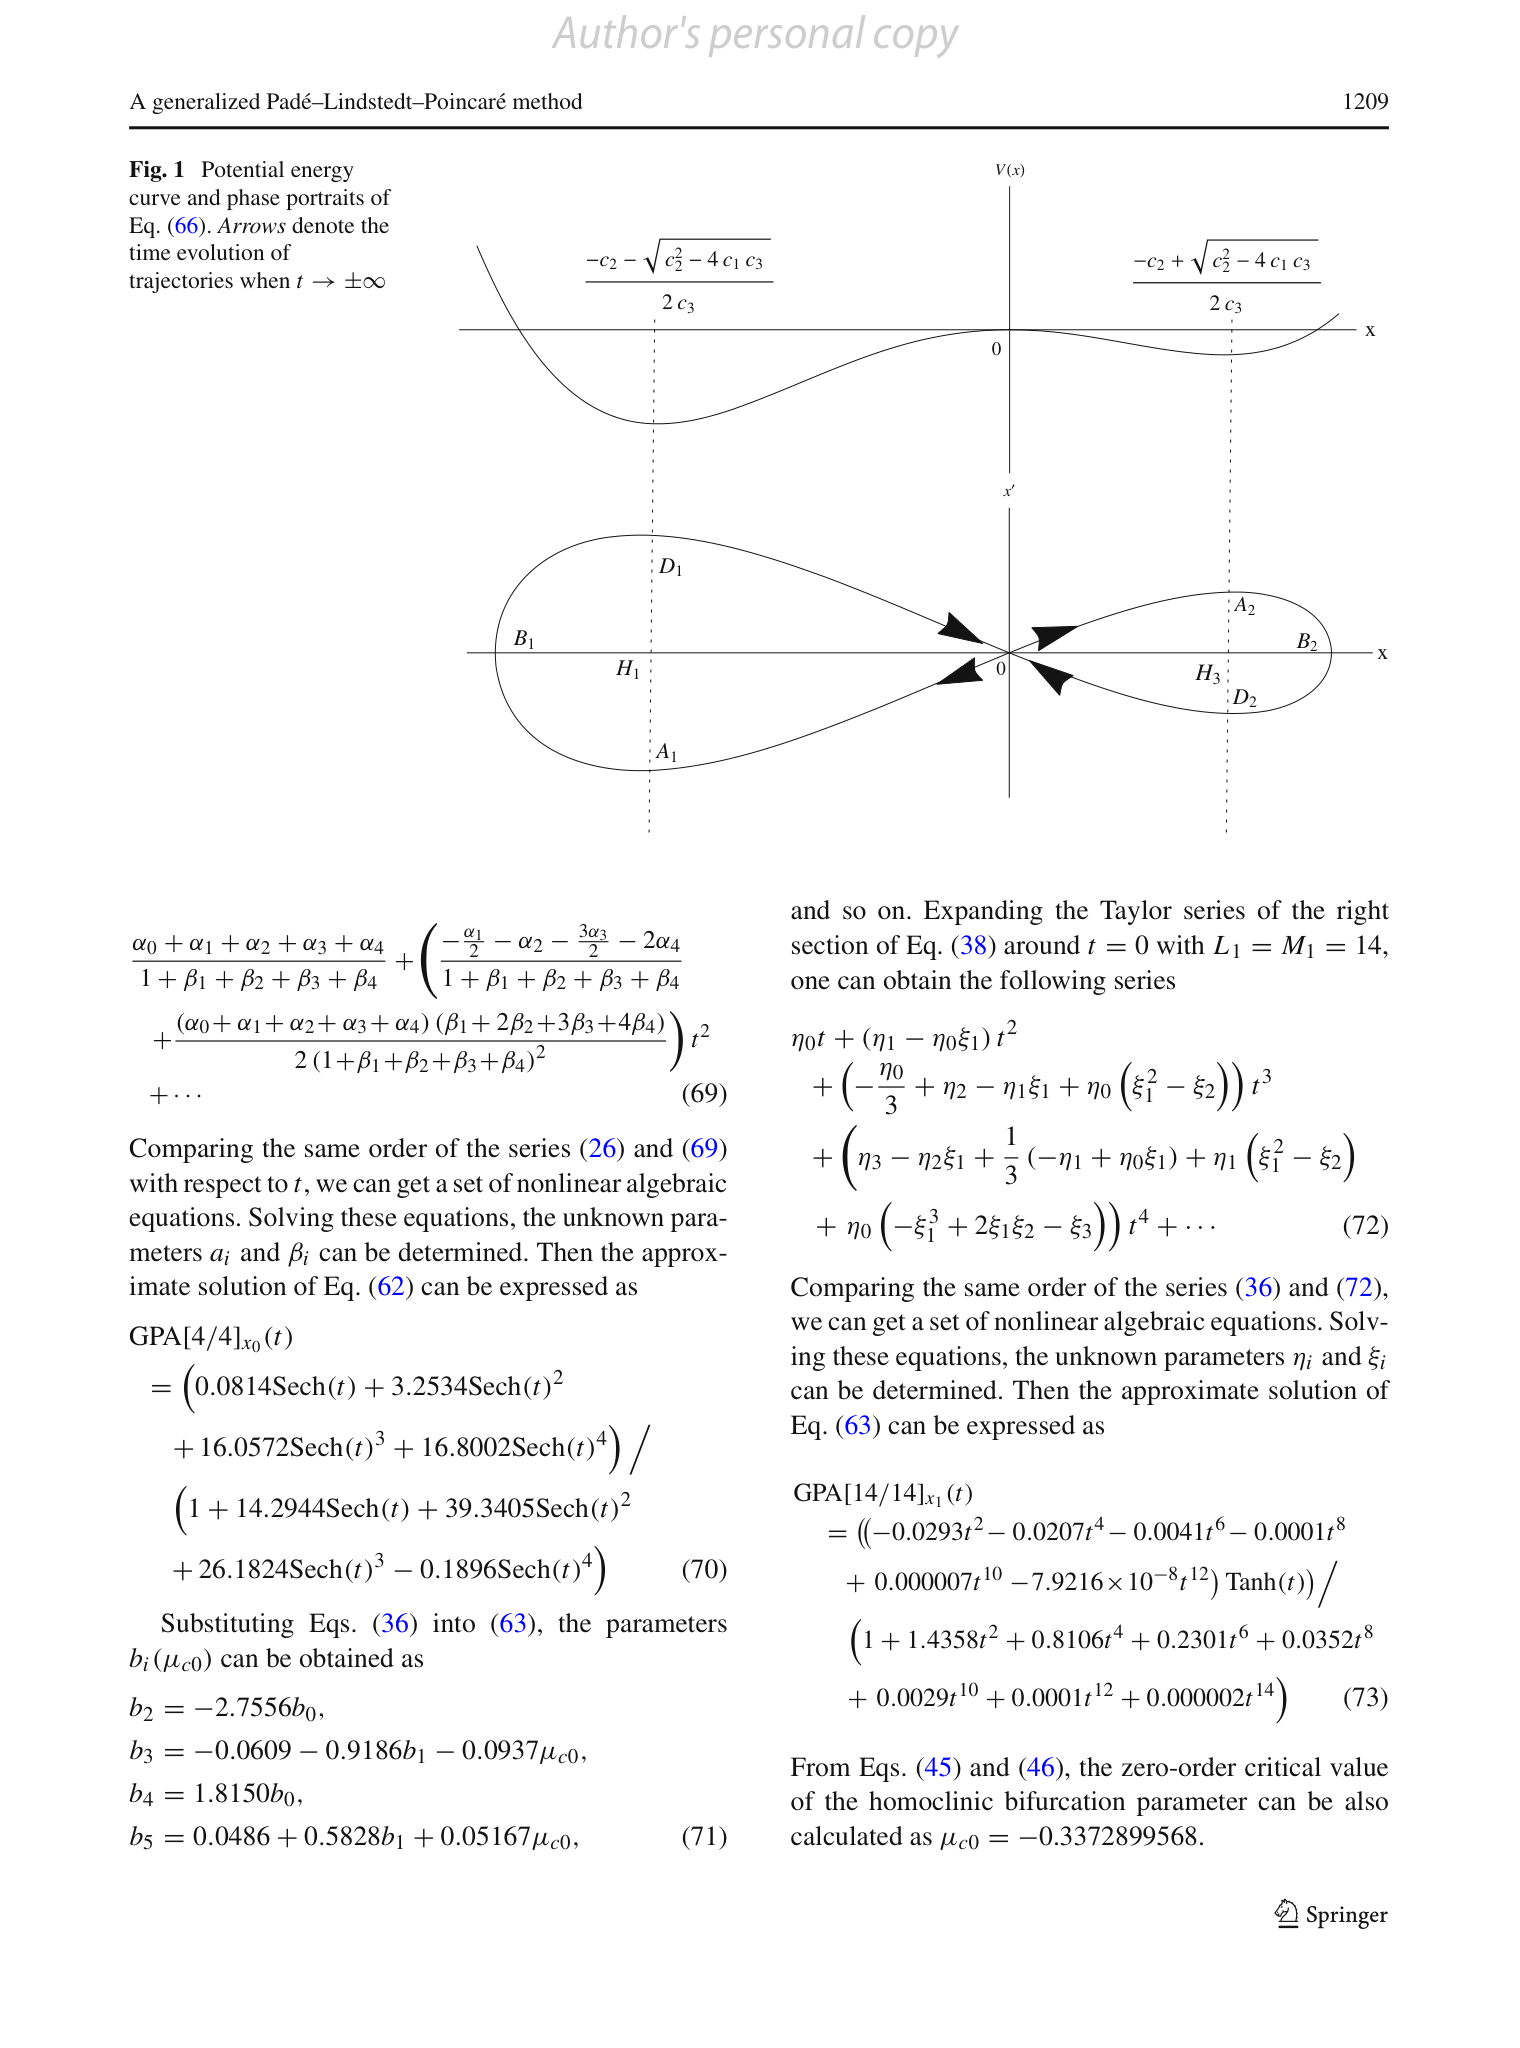
\includegraphics[width=0.85\textwidth,height=0.38\textheight,keepaspectratio]{p10-fig1.png}
\caption{Potential energy curve and phase portraits for the Helmholtz--Duffing oscillator.}
\end{figure}

\subsection{Duffing-Harmonic Oscillator}

For oscillators with rational restoring forces, GPLP handles homoclinic orbits under both small ($\varepsilon = 0.05$) and moderate ($\varepsilon = 0.1$) perturbation parameters (Fig.\ 3).

\begin{figure}[htbp]
\centering
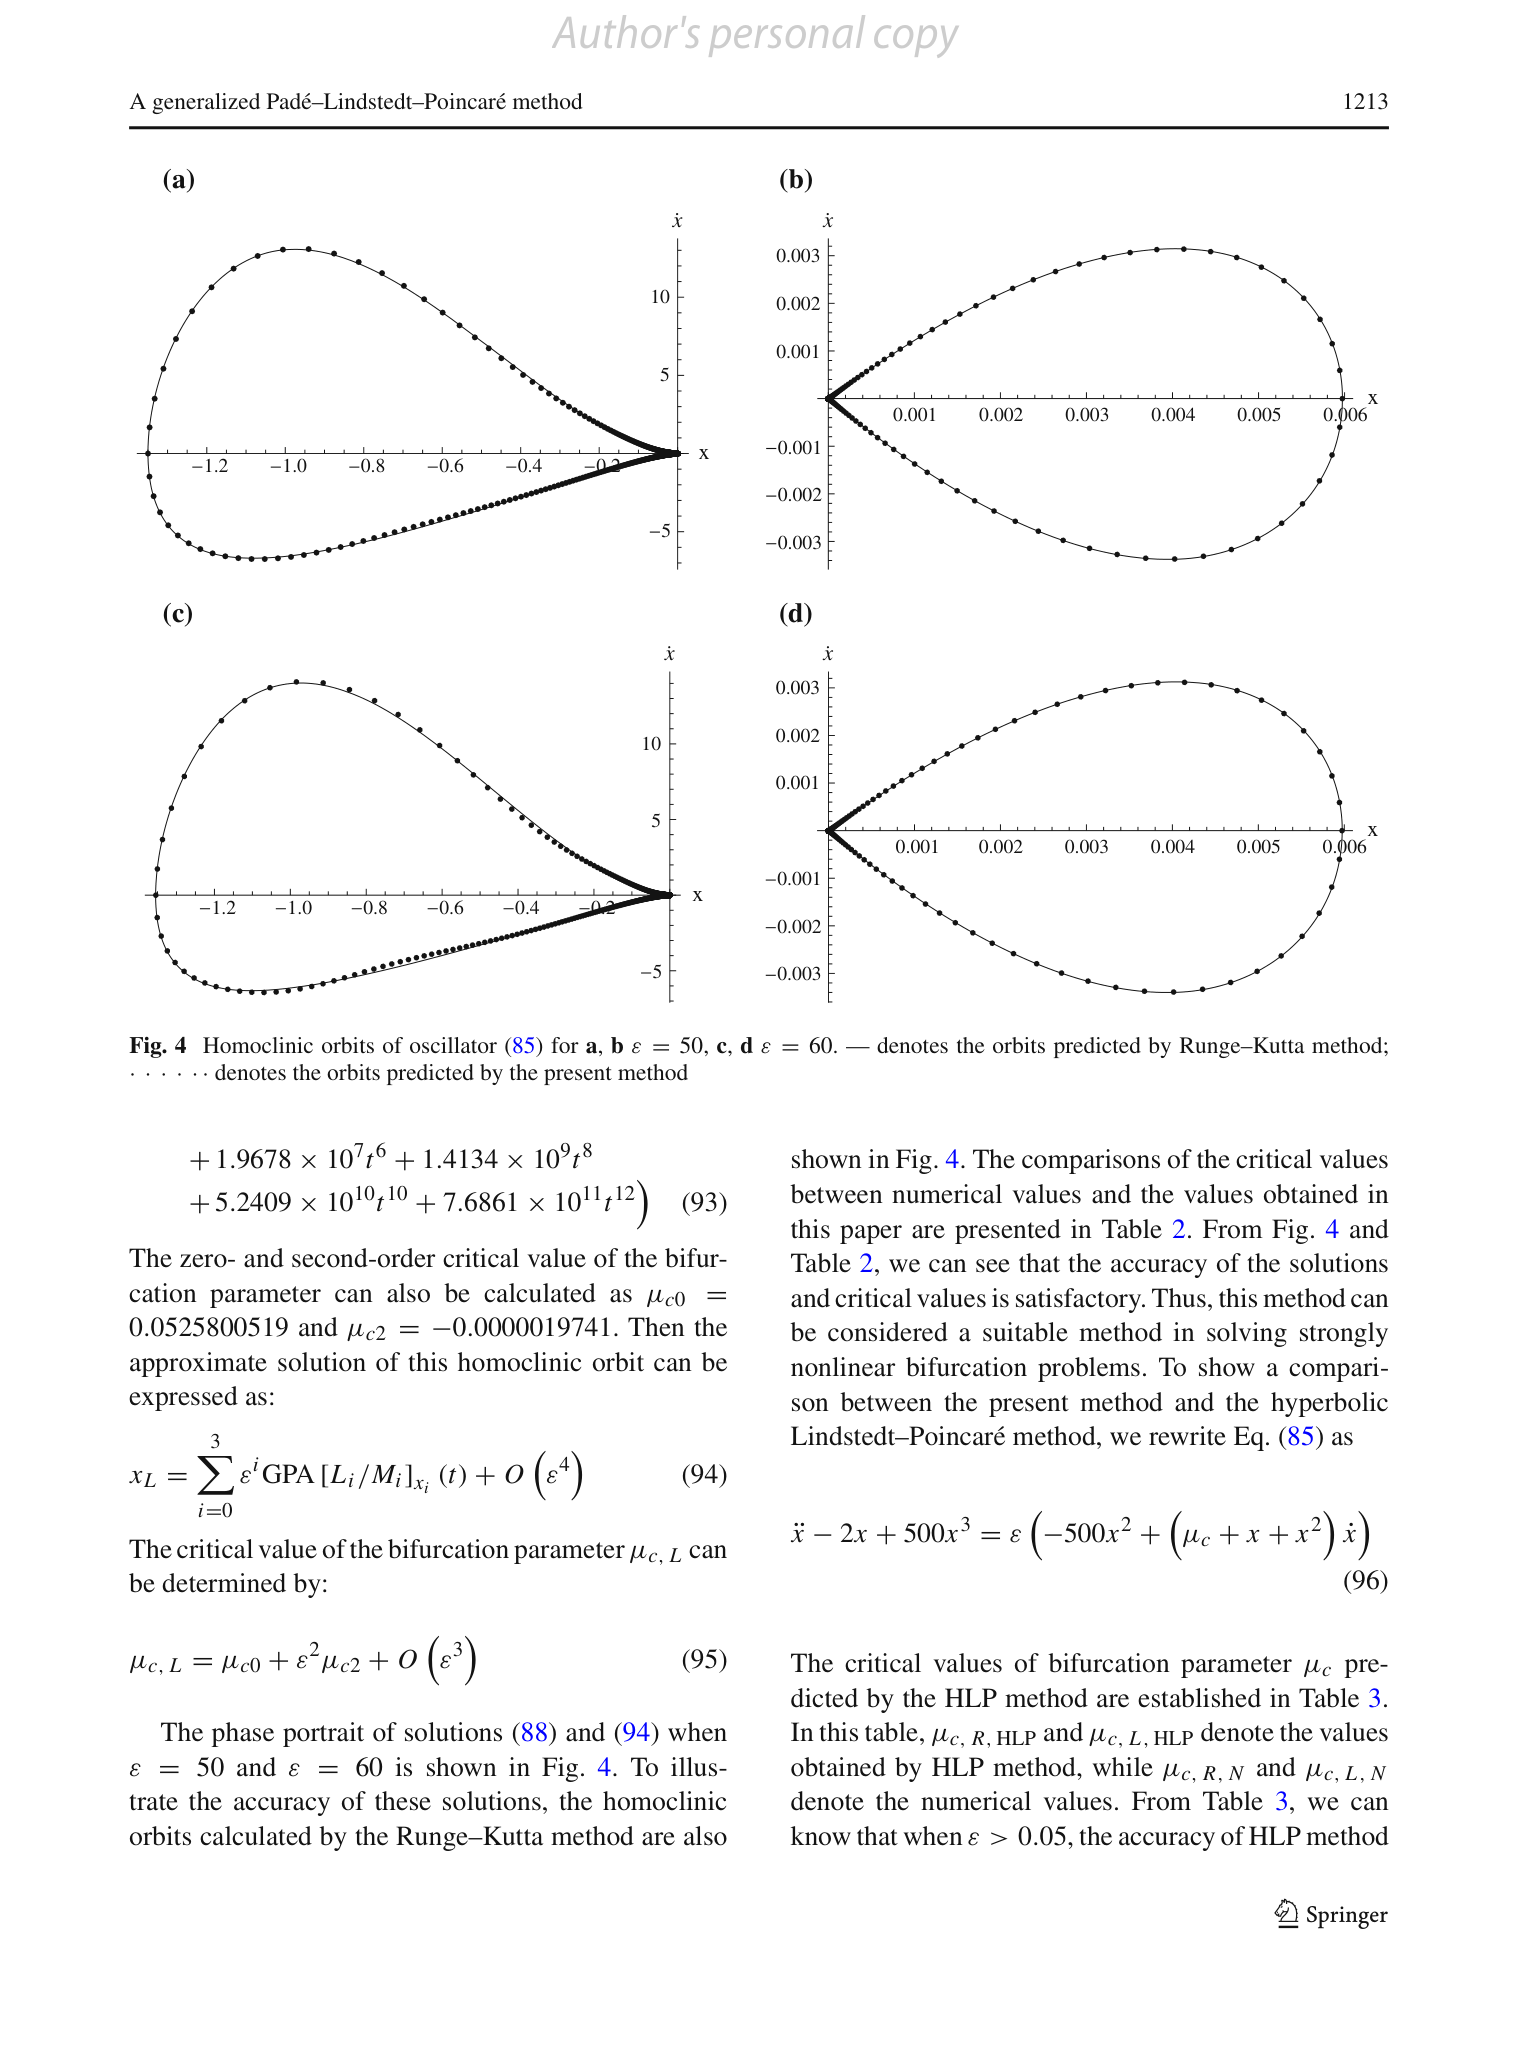
\includegraphics[width=0.85\textwidth,height=0.38\textheight,keepaspectratio]{p10-fig3.png}
\caption{Homoclinic orbits of the Duffing-harmonic oscillator for $\varepsilon=0.05$ (a) and $\varepsilon=0.1$ (b). Solid: Runge--Kutta. Dashed: GPLP.}
\end{figure}

\subsection{SD Oscillator (Multi-Well)}

The irrational SD oscillator is the most challenging test case. GPLP successfully predicts homoclinic orbits in both double-well and triple-well configurations (Figs.\ 4--5).

\begin{figure}[htbp]
\centering
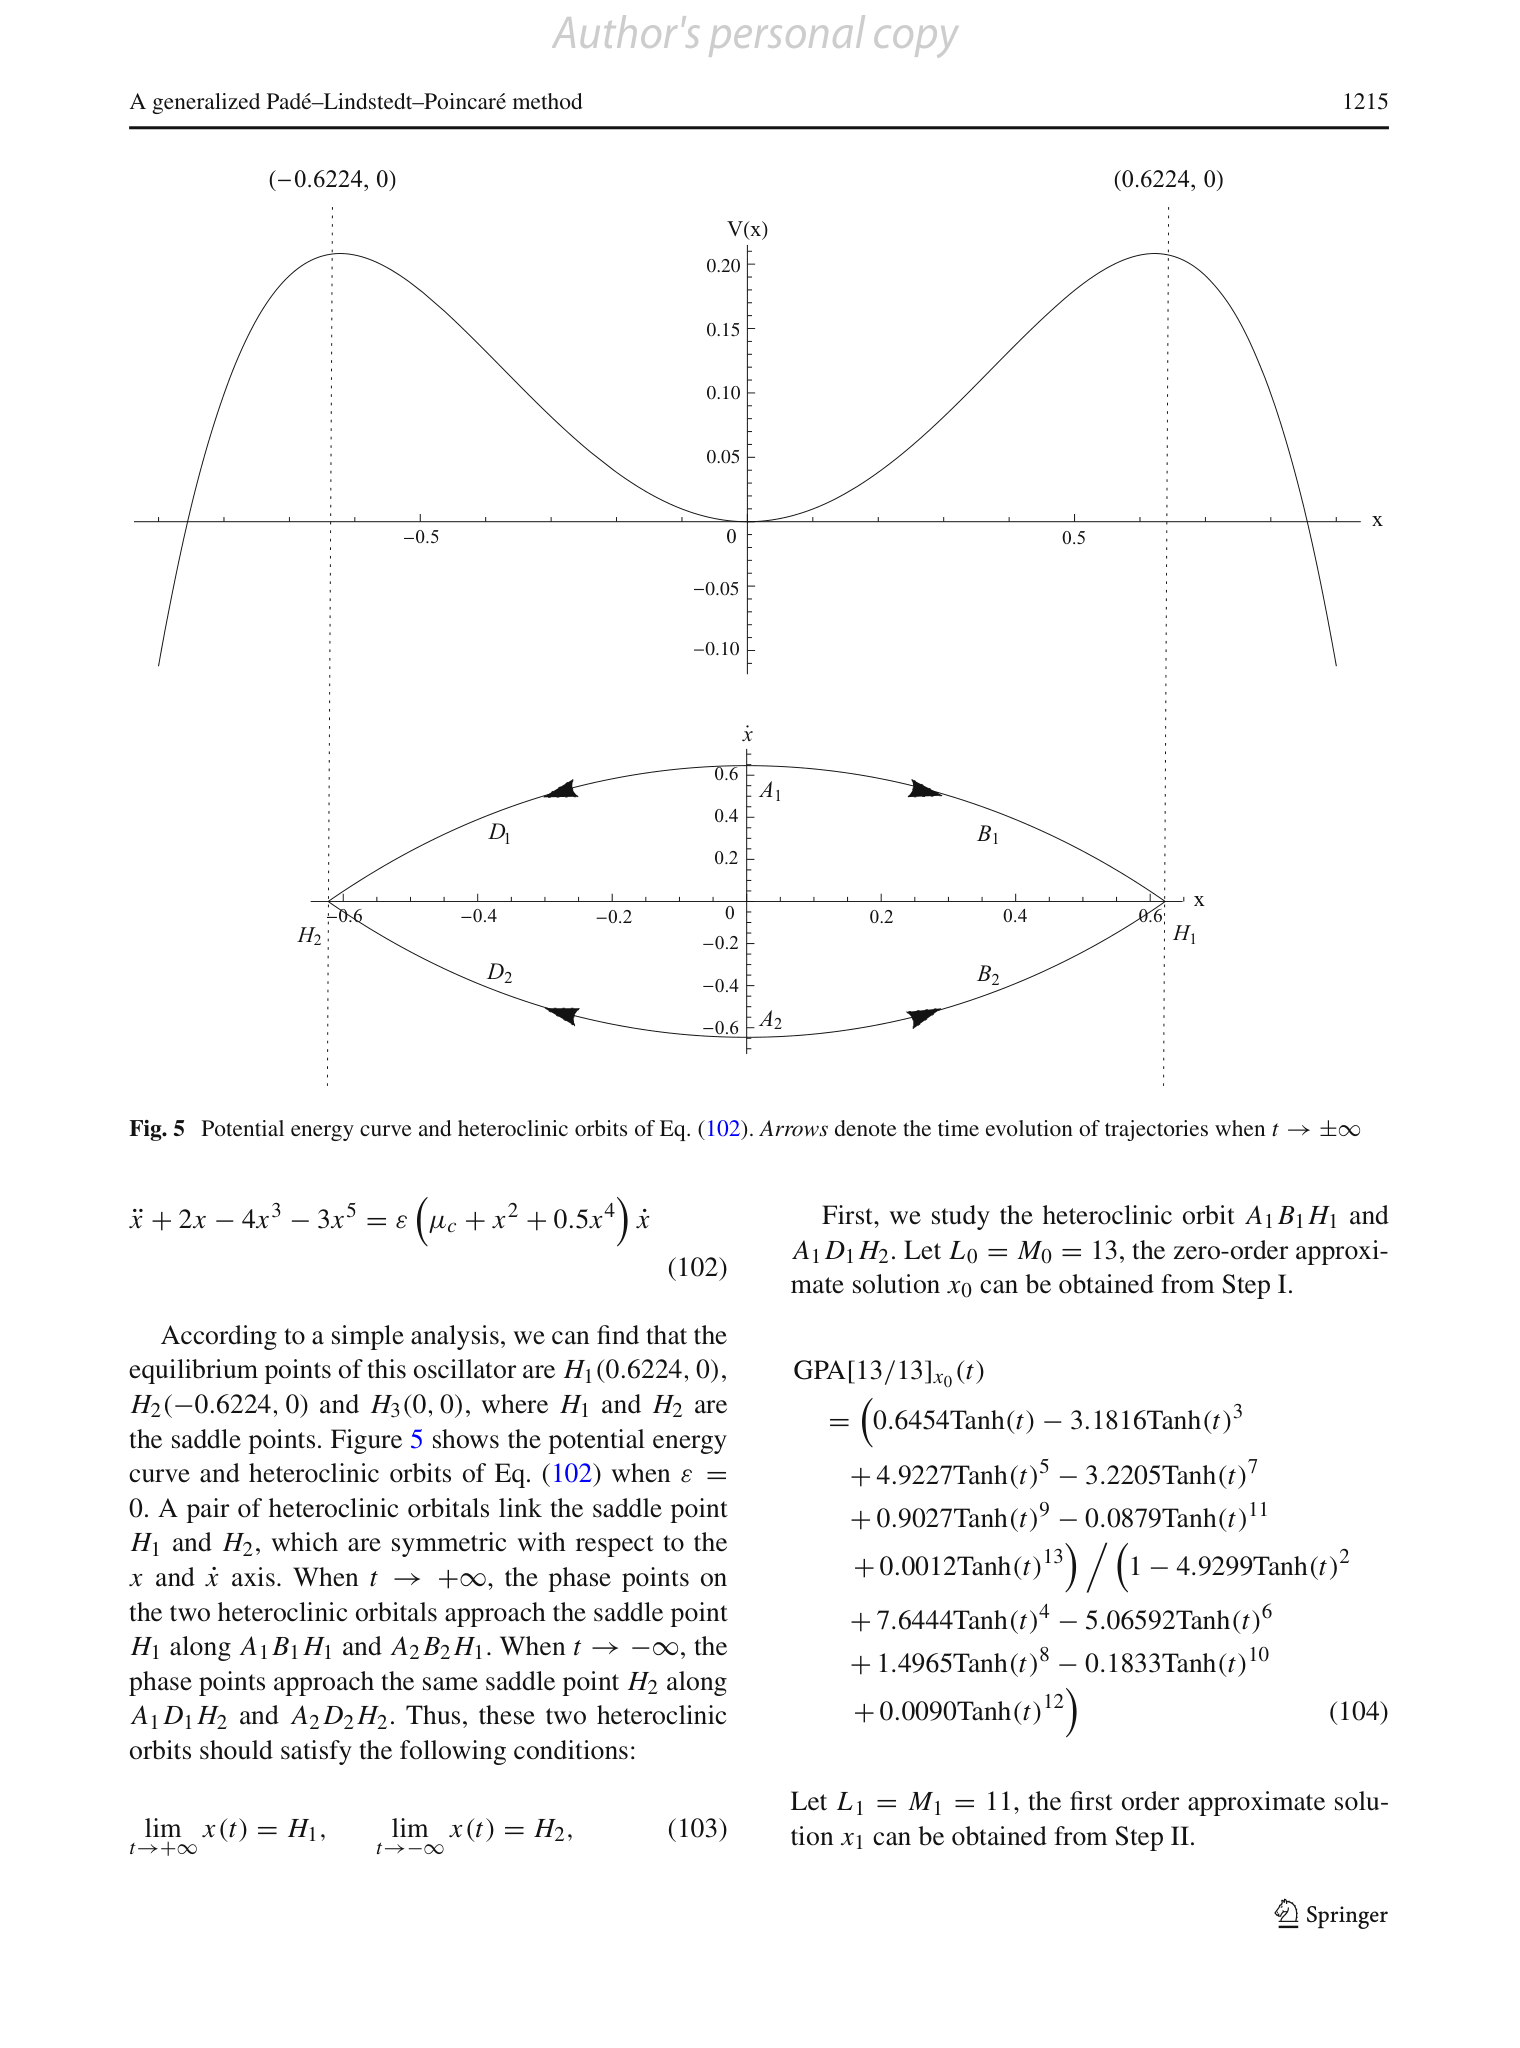
\includegraphics[width=0.85\textwidth,height=0.38\textheight,keepaspectratio]{p10-fig4.png}
\caption{Homoclinic orbits of the SD oscillator at large perturbation parameters ($\varepsilon=50$, 60).}
\end{figure}

\subsection{Simultaneous Homo-Heteroclinic Prediction}

For oscillators where both homoclinic and heteroclinic orbits coexist at the same saddle (e.g., certain parameter regions of the DH-VDP oscillator), GPLP predicts \textbf{both critical parameter values simultaneously} (Fig.\ 12), a capability not available from standard perturbation methods.

\section{Key Findings}

\begin{enumerate}[leftmargin=2em]
\item \textbf{No-integration perturbation method:} GPLP eliminates the derivation/integration bottleneck of classical L--P, enabling high-order solutions for complicated oscillators.
\item \textbf{Multiple approximant types:} Different generalized Pad\'e approximants are tailored to symmetric homoclinic, asymmetric heteroclinic, and mixed-mode orbits.
\item \textbf{Wide applicability:} Validated on Helmholtz--Duffing (polynomial), Duffing-harmonic (rational), and SD (irrational) oscillators.
\item \textbf{Simultaneous bifurcation prediction:} For the first time, both homoclinic and heteroclinic bifurcation parameters are predicted analytically in a unified framework.
\end{enumerate}

\vfill
\begin{center}
\small\rule{0.5\textwidth}{0.3pt}\\[4pt]
\small\color{primary} Author: Zhenbo Li (lizhenbo@usc.edu.cn)\\
\small University of South China, School of Mathematics and Physics
\end{center}

\end{document}
